\section{Internal Block Diagram - AU2}
\label{sec:IBDAU2}
The IBD on \ref{fig:IBD} shows the internal connection between the blocks described in the BDD. As both BMS and MCS are large and complicated blocks they are simplified as single blocks in this IBD. The internal connections of the BMS and MCS are described using separate IBD's in later sections and the IBD below should only be used to gain a general overview of the system's internal connectivity. 

\begin{figure}[H]
	\centering
	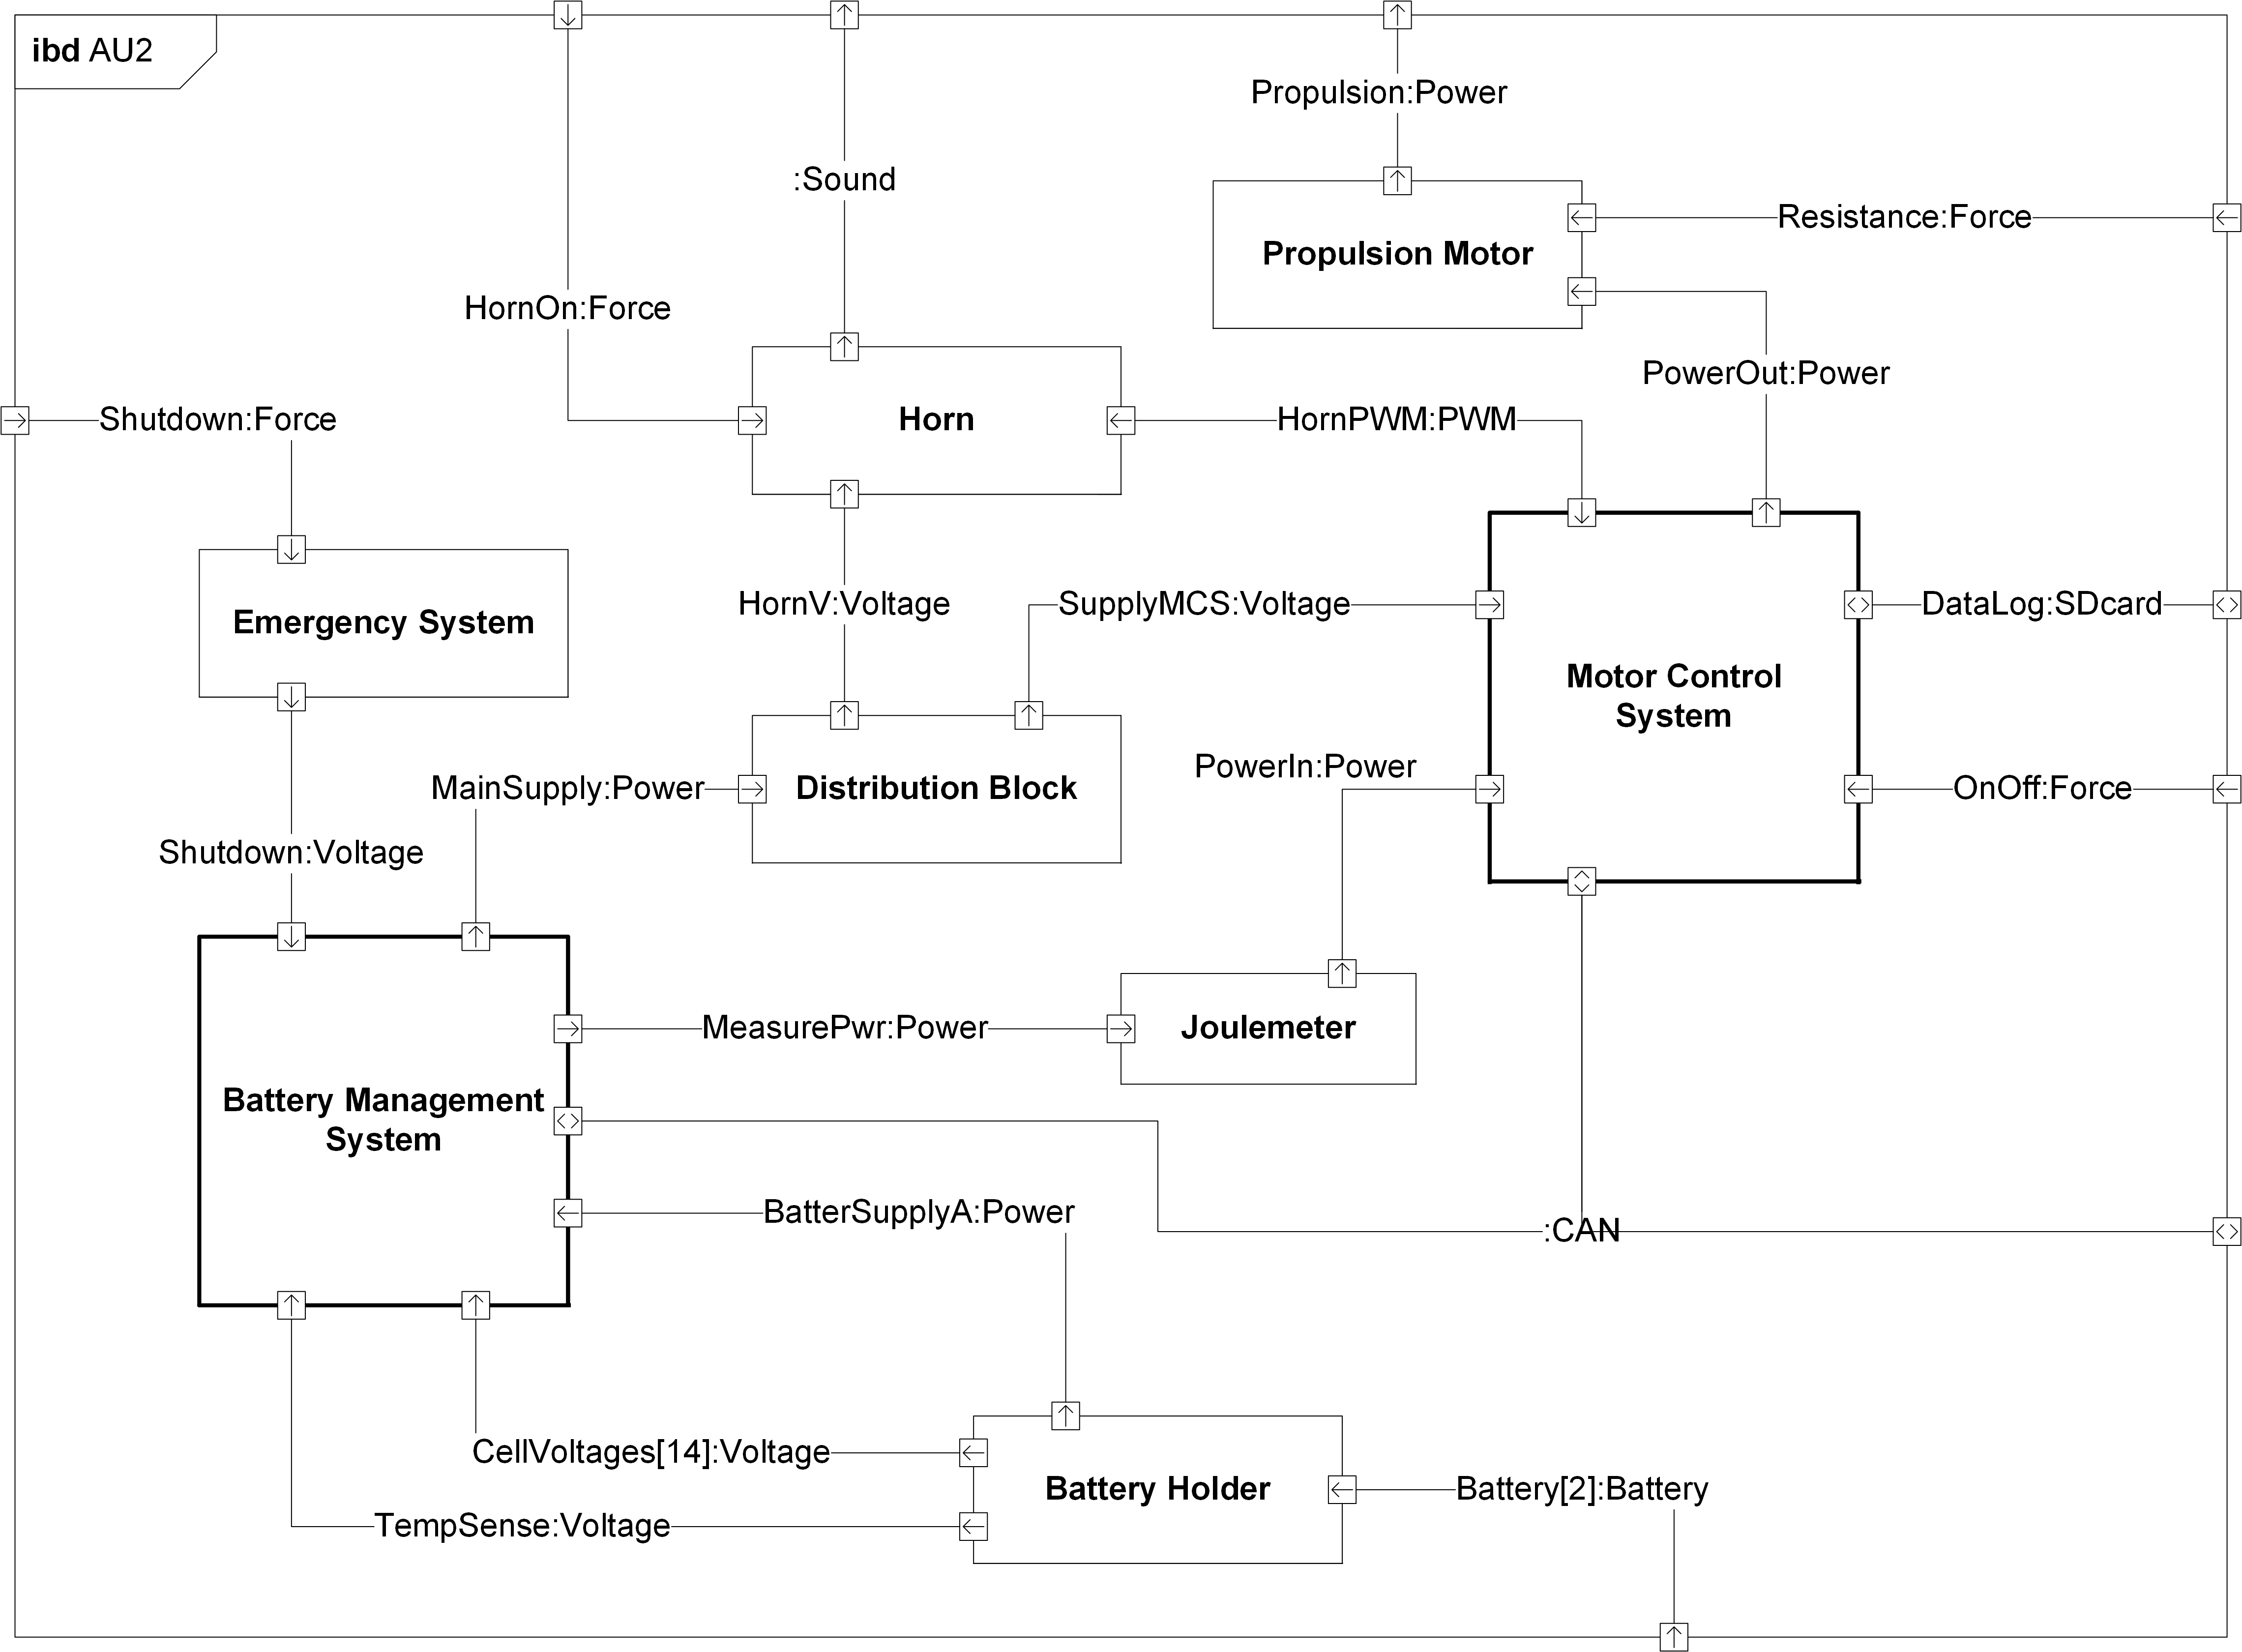
\includegraphics[width=1\linewidth]{Architecture/Diagrams/IBD_AU2}
	\caption{IBD for AU2}
	\label{fig:IBD}
\end{figure}

As the Joulemeter is only part of the system during SEM it is not a vital block. During times where the Joulemeter isn't implemented the block's input/output should simply be connected to eachother.

%The connection MotorPower:PowerMeas should only be used when AU2 is connected with Rolling Road for testing purposes. This is represented by a dotted connector. 